%%%%%%%%%%%%%%%%%%%%%%%%%%%%%%%%%%%%%%%%%%%%%%%%%%%%%%%
%% Modelo LaTeX de monografia UCS                    %%
%% Data de Modificação: 10 de agosto de 2021         %%
%%                                                   %%
%%%%%%%%%%%%%%%%%%%%%%%%%%%%%%%%%%%%%%%%%%%%%%%%%%%%%%%

% ---
\documentclass[
	12pt,				% tamanho da fonte
	openright,			% capítulos começam em pág ímpar (insere página vazia caso preciso)
	oneside,			% para impressão em uma folha. Oposto a twoside
	a4paper,			% tamanho do papel. 
	% -- opções do pacote babel --
	english,			% idioma adicional para hifenização
	french,				% idioma adicional para hifenização
	spanish,			% idioma adicional para hifenização
	brazil				% o último idioma é o principal do documento
	]{abntex2}

% ---
% Pacotes básicos 
% ---
\usepackage[table]{xcolor}
\usepackage{adjustbox}
\usepackage{amsmath}
\usepackage{chemformula} 
\usepackage{chemfig} 
\usepackage{mathtools}
\usepackage{float}
\usepackage[printonlyused]{acronym}

\usepackage{setspace}

\usepackage{times}
\usepackage[T1]{fontenc}		% Seleção de codigos de fonte.
\usepackage[utf8]{inputenc}		% Codificação do documento (conversão automática dos acentos)
\usepackage{lastpage}			% Usado pela Ficha catalográfica
\usepackage{indentfirst}		% Indenta o primeiro parágrafo de cada seção.
\usepackage{color}				% Controle das cores
\usepackage{graphicx}			% Inclusão de gráficos
\usepackage{subcaption}
\usepackage{ragged2e}
%\usepackage{microtype} 			% para melhorias de justificação

\usepackage[alf,
            versalete,
            abnt-emphasize = bf,                % destaca o titulo em negrito;
            abnt-etal-list = 3,                 % trabalhos com mais de 3 autores recebem et al.,;
            abnt-etal-text = it,                % escreve o et al., em itálico;
            abnt-and-type = e,                 % usa o caractere 'e' para mais de um autor;
            abnt-last-names = abnt,             % trata sobrenomes 'estritamente' conforme a ABNT; e
            abnt-repeated-author-omit = yes     % autores com + de uma entrada recebem '____.'
]{abntex2cite}

% pacotes de tabelas
\usepackage{multicol}	% Suporte a mesclagens em colunas
\usepackage{multirow}	% Suporte a mesclagens em linhas
\usepackage{longtable}	% Tabelas com várias páginas
\usepackage{fr-longtable, ltcaption}% permitir adicionar conclusão na última página de longtable
\usepackage{threeparttablex}    % notas no longtable
\renewcommand\tabularxcolumn[1]{m{#1}} % for vertical centering text in X column
\usepackage{array}

\usepackage{listings}
\usepackage{hyperref}

\AtBeginDocument{% the counter is defined later
  \counterwithout{lstlisting}{chapter}%
}
\makeatletter
\renewcommand{\l@lstlisting}[2]{%
  \@dottedtocline{1}{0em}{1.5em}{\lstlistingname\ #1}{#2}%
}

\renewcommand{\lstlistingname}{Algoritmo}% Listing -> Algorithm
\renewcommand{\lstlistlistingname}{LISTA DE ALGORITMOS}% List of Listings -> List of Algorithms

\usepackage{pgfplots} %graficos
\usepackage{booktabs,makecell}
\usepackage{siunitx}

\usepackage{array}

\newcolumntype{L}[1]{>{\raggedright\let\newline\\\arraybackslash\hspace{0pt}}m{#1}}
\newcolumntype{C}[1]{>{\centering\let\newline\\\arraybackslash\hspace{0pt}}m{#1}}
\newcolumntype{R}[1]{>{\raggedleft\let\newline\\\arraybackslash\hspace{0pt}}m{#1}}

%=======================================================================
% CONFIGURAÇÕES DE PACOTES
%=======================================================================
\DeclareMathOperator*{\maxi}{Maximizar}
\DeclareMathOperator*{\mini}{Minimizar }

\newcommand{\icol}[1]{% inline column vector
  \left(\begin{smallmatrix}#1\end{smallmatrix}\right)%
}

%------
% Configurações dos Algoritmos/Código
%------
\lstset{language=C,                 % linguagem padrão (pode ser modificada em cada algoritmo/código)   
        basicstyle=\footnotesize,   % tamanho da fonte utilizado para o código
        numbers=left,               % onde colocar os números da linha
        numberstyle=\footnotesize,  %estilo a ser utilizado pelos números
        frame=single                % adiciona um quadro ao redor do código
} 

%=======================================================================
% Informações de dados para CAPA, FOLHA DE ROSTO e FOLHA DE APROVAÇÃO
%=======================================================================
\titulo{LOTUS - Solução Distribuída para o Gerenciamento Eficiente de Ativos de TI}
\autor{
    Arthur Gonçalves \\
    Bruno Gonçalves Martins \\
    Marco Aurélio da Rosa Haubrich \\
    Samuel Frederico
}
\local{Caxias do Sul}
\data{2024}
\orientador{Prof.}

\universidade{UNIVERSIDADE DE CAXIAS DO SUL}
\area{ÁREA DO CONHECIMENTO DE CIÊNCIAS EXATAS E ENGENHARIAS}
\preambulo{
  Projeto de Pesquisa apresentado como parte dos requisitos da disciplina Laboratório de Software nos cursos de Engenharia de Software, Análise e Desenvolvimento de Sistemas e Ciência da Computação na Universidade de Caxias do Sul.
}

\tipotrabalho{Projeto de Pesquisa}
% ---

% alterando o aspecto da cor azul
\definecolor{blue}{RGB}{41,5,195}

% informações do PDF
\makeatletter
\hypersetup{
     	%pagebackref=true,
		pdftitle={\@title}, 
		pdfauthor={\@author},
    	pdfsubject={\imprimirpreambulo},
	    pdfcreator={LaTeX with abnTeX2},
		pdfkeywords={abnt}{latex}{abntex}{abntex2}{trabalho acadêmico}, 
		colorlinks=true,       		% false: boxed links; true: colored links
    	linkcolor=black,          	% color of internal links
    	citecolor=black,        	% color of links to bibliography
    	filecolor=magenta,      	% color of file links
		urlcolor=black,
		bookmarksdepth=4
}
\makeatother
% --- 

% ---
% Posiciona figuras e tabelas no topo da página quando adicionadas sozinhas
% em um página em branco. Ver https://github.com/abntex/abntex2/issues/170
\makeatletter
\setlength{\@fptop}{5pt} % Set distance from top of page to first float
\makeatother
% ---

% ---% Possibilita criação de Quadros e Lista de quadros.
% Ver https://github.com/abntex/abntex2/issues/176
%
\newcommand{\quadroname}{Quadro}
\newcommand{\listofquadrosname}{Lista de quadros}

%\newfloat[chapter]{quadro}{loq}{\quadroname}
\newlistof{listofquadros}{loq}{\listofquadrosname}
\newlistentry{quadro}{loq}{0}

% configurações para atender às regras da ABNT
\setfloatadjustment{quadro}{\centering}
\counterwithout{quadro}{chapter}
\renewcommand{\cftquadroname}{\quadroname\space} 
\renewcommand*{\cftquadroaftersnum}{\hfill--\hfill}

\setfloatlocations{quadro}{hbtp} % Ver https://github.com/abntex/abntex2/issues/176
% --- 
% Espaçamentos entre linhas e parágrafos 
% --- 

% O tamanho do parágrafo é dado por:
\setlength{\parindent}{1.3cm}

% Controle do espaçamento entre um parágrafo e outro:
\setlength{\parskip}{0.2cm}  % tente também \onelineskip

% ---
% compila o índice
% ---
\makeindex
% ---

% ----
% Início do documento
% ----
\pgfplotsset{compat=1.15}
\begin{document}

% Seleciona o idioma do documento (conforme pacotes do babel)
\selectlanguage{brazil}

% Retira espaço extra obsoleto entre as frases.
\frenchspacing 

%=======================================================================
% ELEMENTOS PRÉ-TEXTUAIS
%=======================================================================

% ----------------------------------------------------------------------
% Capa
% ----------------------------------------------------------------------
\imprimircapa

% ----------------------------------------------------------------------
% Folha de rosto
% ----------------------------------------------------------------------
%\imprimirfolhaderosto

% ----------------------------------------------------------------------
% Folha de aprovação
% ----------------------------------------------------------------------
\newpage
%\include{1-pre-textuais/aprovacao}

% ----------------------------------------------------------------------
% Dedicatória (opcional).
% ----------------------------------------------------------------------
%\imprimirdedicatoria{1-pre-textuais/dedicatoria}

% ----------------------------------------------------------------------
% Agradecimentos (opcional).
% ----------------------------------------------------------------------
%\imprimiragradecimentos{1-pre-textuais/agradecimentos}

% ----------------------------------------------------------------------
% Epígrafe (opcional).
% ----------------------------------------------------------------------
%\include{1-pre-textuais/epigrafe}

% ----------------------------------------------------------------------
% Resumo  
% ----------------------------------------------------------------------
% Resumo em Português
\setlength{\absparsep}{18pt} % ajusta o espaçamento dos parágrafos do resumo
\begin{resumo}[RESUMO]
Este projeto apresenta o LOTUS, uma solução distribuída para o gerenciamento de ativos de TI, composta por uma interface desktop, um servidor central e agentes instalados nos dispositivos. O sistema permite rastrear ativos em tempo real, manter históricos de alterações e otimizar a gestão em ambientes complexos. Além de resolver desafios organizacionais, o desenvolvimento focou no aprendizado de arquiteturas em camadas e design patterns, promovendo escalabilidade, usabilidade e boas práticas de desenvolvimento.


% Coloque após os ":"  as palavras-chave com a primeira 
% letra de cada palavra em maiúscula e separadas por ponto.
\textbf{Palavras-chave}: Gerenciamento de Ativos de TI. Arquitetura em Camadas. Sistemas Distribuídos. Padrões de Projeto. Governança de TI. Desenvolvimento de Software.
\end{resumo}


% ----------------------------------------------------------------------
% Abstract 
% ----------------------------------------------------------------------
%\include{1-pre-textuais/abstract}

% ----------------------------------------------------------------------
% Lista de Figuras (se necessário)
% ----------------------------------------------------------------------
\pdfbookmark[0]{\listfigurename}{lof}
%\listoffigures*
\cleardoublepage

% ----------------------------------------------------------------------
% Lista de Tabelas (se necessário)
% ----------------------------------------------------------------------
%\pdfbookmark[0]{\listtablename}{lot}
%\listoftables*
%\cleardoublepage

% ----------------------------------------------------------------------
% Lista de Quadros (se necessário)
% ----------------------------------------------------------------------
%\pdfbookmark[0]{\listofquadrosname}{loq}
%\listofquadros*
%\cleardoublepage

% ----------------------------------------------------------------------
% Lista de Algoritmos (se necessário)
% ----------------------------------------------------------------------
%\newlistof{lstlistoflistings}{lol}{\lstlistlistingname}
%\lstlistoflistings*
%\cleardoublepage

% ----------------------------------------------------------------------
% Lista de abreviaturas e siglas (opcional)
% ----------------------------------------------------------------------
%\include{1-pre-textuais/abreviaturassiglas}

% ----------------------------------------------------------------------
% Lista de símbolos (opcional)
% ----------------------------------------------------------------------
%\include{1-pre-textuais/simbolos}

% ----------------------------------------------------------------------
% Sumário
% ----------------------------------------------------------------------
% \pdfbookmark[0]{\contentsname}{toc}
% \tableofcontents*
% \cleardoublepage

%=======================================================================
% ELEMENTOS TEXTUAIS
%=======================================================================
\textual

\chapter{INTRODUÇÃO}

No cenário atual, a gestão eficiente de ativos de TI é um aspecto essencial para o sucesso das organizações. Com o crescente aumento na quantidade e diversidade de equipamentos, como computadores, impressoras e monitores, o controle desses recursos tornou-se uma tarefa desafiadora, especialmente em empresas de médio e grande porte. A ausência de uma gestão organizada pode levar a problemas como perda de dispositivos, dificuldade em rastrear histórico de alterações e movimentações, além de impactos negativos na produtividade e na tomada de decisão. Por isso, soluções tecnológicas que permitam rastrear, organizar e gerenciar esses ativos são fundamentais para garantir a eficiência operacional e o alinhamento com as práticas modernas de governança de TI.

Neste contexto, o desenvolvimento de soluções como o sistema LOTUS exige a aplicação de metodologias robustas de engenharia de software, que proporcionem escalabilidade, modularidade e manutenção simplificada. A arquitetura em camadas, amplamente utilizada no desenvolvimento de sistemas distribuídos, se destaca por separar as responsabilidades em diferentes níveis, como interface do usuário, lógica de negócio e acesso a dados, garantindo maior organização e clareza no código.

Adicionalmente, o uso de padrões de projeto (design patterns) desempenha um papel crucial na criação de sistemas eficientes e bem estruturados. Esses padrões oferecem soluções testadas para problemas recorrentes no desenvolvimento de software, promovendo a reutilização de código, a redução de complexidade e a facilidade de manutenção. Ao combinar esses dois conceitos, arquitetura em camadas e padrões de projeto, é possível desenvolver sistemas mais robustos, escaláveis e alinhados às melhores práticas da indústria, como demonstrado no projeto LOTUS.

\section{Arquitetura em Camadas}

A arquitetura em camadas é um modelo amplamente utilizado no desenvolvimento de software para organizar e estruturar sistemas em módulos independentes, facilitando a manutenção, a escalabilidade e a reutilização do código. Essa abordagem divide as responsabilidades do sistema em diferentes camadas, cada uma desempenhando um papel específico, como interface com o usuário, lógica de negócio e acesso a dados. Essa separação clara de responsabilidades promove maior modularidade e facilita o desenvolvimento colaborativo, além de permitir a substituição ou atualização de componentes individuais sem impactar significativamente outras partes do sistema \cite{bass2003}.

Entre os modelos mais comuns de arquitetura em camadas estão o \textit{Model-View-Controller} (MVC) e a arquitetura \textit{N-tier}. Ambos apresentam características distintas que os tornam adequados para diferentes tipos de projetos.

\subsection{Modelo MVC (Model-View-Controller)}

O padrão \textit{Model-View-Controller} (MVC) é uma abordagem popular para a organização de aplicações com base na separação de responsabilidades. Ele divide o sistema em três componentes principais:

\begin{itemize}
    \item \textbf{Model}: Representa os dados e as regras de negócio do sistema. É responsável por acessar e gerenciar as informações armazenadas, além de implementar a lógica que governa as operações desses dados \cite{fowler2003}.
    \item \textbf{View}: Trata da interface com o usuário, exibindo as informações do \textit{Model} e capturando as interações realizadas pelo usuário.
    \item \textbf{Controller}: Atua como intermediário entre o \textit{Model} e a \textit{View}, processando as entradas do usuário e coordenando as respostas apropriadas por meio da atualização dos dados ou da interface.
\end{itemize}

Essa separação permite que cada componente seja desenvolvido e testado independentemente, promovendo maior flexibilidade e manutenção do sistema. Segundo Fowler \cite{fowler2003}, o padrão MVC é fundamental para aplicações que requerem interfaces de usuário dinâmicas e frequentemente atualizadas, permitindo a escalabilidade e a adaptação às mudanças tecnológicas.

\subsection{Arquitetura N-tier}

A arquitetura \textit{N-tier} é uma extensão da ideia de separação de camadas, frequentemente utilizada em sistemas distribuídos. Ela organiza o sistema em múltiplas camadas, sendo as mais comuns:

\begin{itemize}
    \item \textbf{Camada de Apresentação (Presentation Layer)}: Responsável pela interação com o usuário, como interfaces gráficas ou APIs.
    \item \textbf{Camada de Aplicação ou Negócio (Business Logic Layer)}: Contém a lógica de negócio, processando as regras e operações do sistema \cite{richards2015}.
    \item \textbf{Camada de Dados (Data Layer)}: Gerencia o acesso e a manipulação dos dados armazenados, geralmente em bancos de dados.
\end{itemize}

O termo \textit{N-tier} refere-se à possibilidade de adicionar outras camadas especializadas, como uma camada de serviços ou \textit{middleware}, dependendo da complexidade do sistema. Essa arquitetura é ideal para sistemas escaláveis e distribuídos, já que cada camada pode ser executada em servidores diferentes, permitindo a distribuição de carga e o aumento da robustez \cite{bass2003}.

\section{Introdução aos Design Patterns}

Os \textit{Design Patterns} (Padrões de Projeto) são soluções reutilizáveis para problemas recorrentes no desenvolvimento de software. Eles representam boas práticas organizadas e documentadas, que ajudam a criar sistemas mais flexíveis, escaláveis e fáceis de manter. A aplicação de padrões de projeto permite que desenvolvedores evitem reinventar soluções e se beneficiem de estratégias comprovadas para lidar com desafios de design e implementação \cite{gamma1994}.

Segundo Gamma et al. \cite{gamma1994}, um \textit{Design Pattern} é composto por quatro elementos principais:

\begin{itemize}
    \item \textbf{Nome (Name)}: Um identificador único que descreve o padrão e facilita sua referência.
    \item \textbf{Problema (Problem)}: O contexto e as circunstâncias em que o padrão pode ser aplicado, incluindo os problemas que resolve.
    \item \textbf{Solução (Solution)}: A descrição abstrata de como resolver o problema, incluindo componentes, relações e interações.
    \item \textbf{Consequências (Consequences)}: Os resultados e trocas (trade-offs) associados ao uso do padrão, como benefícios e limitações.
\end{itemize}

Os padrões de projeto são geralmente categorizados em três grupos principais, de acordo com o tipo de problema que resolvem:

\begin{itemize}
    \item \textbf{Padrões Criacionais (Creational Patterns)}: Focados na criação de objetos de maneira flexível e independente de sua implementação. Exemplos incluem o padrão \textit{Singleton} e o \textit{Factory Method}.
    \item \textbf{Padrões Estruturais (Structural Patterns)}: Tratam da composição de classes e objetos para formar estruturas maiores. Exemplos incluem \textit{Adapter} e \textit{Composite}.
    \item \textbf{Padrões Comportamentais (Behavioral Patterns)}: Relacionados à interação e comunicação entre objetos. Exemplos incluem \textit{Observer} e \textit{Strategy}.
\end{itemize}

A adoção de \textit{Design Patterns} não apenas simplifica o desenvolvimento, mas também facilita a comunicação entre desenvolvedores, uma vez que os padrões servem como uma linguagem comum para descrever soluções \cite{gamma1994}.










\section{Objetivo}

O principal objetivo deste projeto é desenvolver o LOTUS, uma solução distribuída para o gerenciamento eficiente de ativos de TI, com foco na organização e rastreabilidade de equipamentos como computadores, impressoras e monitores em empresas de médio e grande porte. A proposta busca facilitar a identificação, localização e monitoramento desses recursos, incluindo a manutenção de um histórico detalhado de alterações e movimentações, promovendo maior controle e eficiência na gestão de TI.

Além de atender a um caso prático de necessidade empresarial, o projeto também possui objetivos acadêmicos e técnicos. Ele visa explorar e aplicar conceitos avançados de engenharia de software, como arquitetura em camadas e \textit{Design Patterns}, para garantir modularidade, escalabilidade e manutenção simplificada do sistema. Esses conceitos foram integrados de maneira a proporcionar uma melhor compreensão das boas práticas de desenvolvimento e do uso de soluções arquiteturais na construção de sistemas complexos.

O projeto também objetiva contribuir para a capacitação técnica da equipe envolvida, promovendo o aprendizado prático de tecnologias e metodologias de desenvolvimento de software. Ao final, espera-se que o LOTUS não apenas atenda às demandas do caso real que o originou, mas também sirva como uma base sólida para futuros aprimoramentos e aplicações em diferentes contextos empresariais.

\chapter{Modelagem do Sistema}

Neste capítulo, apresentamos a modelagem do sistema, detalhando sua infraestrutura e o fluxo de dados entre os diferentes componentes. A modelagem inclui a interação do usuário com a interface de gerenciamento, a comunicação com o servidor central e a coleta de dados realizada pelos agentes instalados nos dispositivos monitorados. A Figura \ref{fig:Infrasis1} ilustra a infraestrutura completa, destacando o fluxo de informações desde o usuário até os bancos de dados centralizados, garantindo a rastreabilidade e integridade das informações.


\begin{figure}[h]
    \centering
    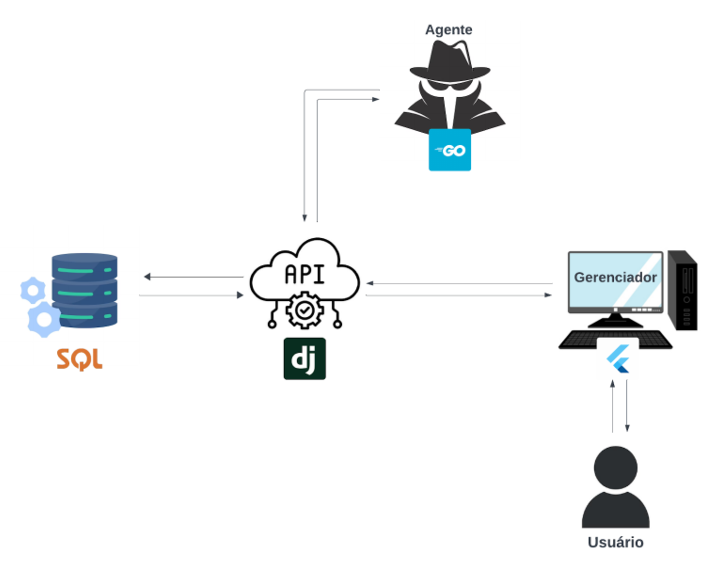
\includegraphics[width=1\linewidth]{figuras/modelagemArc.png}
    \caption{Arquitetura da infraestrutura do sistema}
    \label{fig:Infrasis1}
\end{figure}
Além disso, discutiremos a estruturação do trabalho, incluindo o backlog, o diagrama de classes. A seguir, detalhamos o processo de desenvolvimento e as tecnologias básicas utilizadas para construir nosso sistema.

\section{Planejamento do Desenvolvimento}

Para a construção do sistema, adotamos uma abordagem modular, dividindo o desenvolvimento em três principais componentes: Interface de Gerenciamento Desktop, Servidor Central e Agentes Distribuídos. Cada componente foi cuidadosamente planejado para atender aos requisitos de escalabilidade, eficiência e segurança.  

A interface de gerenciamento foi projetada para oferecer uma experiência de usuário intuitiva, facilitando a visualização e o controle dos ativos. O servidor central foi planejado para gerenciar o armazenamento e o processamento de dados de maneira segura e confiável. Por fim, os agentes distribuídos foram desenvolvidos para capturar informações diretamente dos dispositivos monitorados e comunicar essas informações ao servidor.  

Optamos por definir as tecnologias e frameworks ao longo do processo de implementação, permitindo maior flexibilidade para adaptar as escolhas às necessidades específicas de cada componente e garantir um desempenho otimizado do sistema.


\section{Requisitos de Referência}
Elaboramos uma lista de requisitos para servir como referência na construção do projeto, definindo as principais funcionalidades e características necessárias para atender às demandas identificadas.
\subsection{Requisitos de Negócio}
\begin{itemize}
    \item RN1: O sistema deve otimizar a gestão de ativos de TI, reduzindo o tempo necessário para localizar, atualizar ou consultar informações sobre os equipamentos.
    \item RN2: O sistema deve centralizar todas as informações sobre ativos de TI, incluindo dados de localização, usuários e licenças de software, para facilitar a tomada de decisão.
    \item RN3: O sistema deve permitir um monitoramento em tempo real dos ativos de TI, possibilitando a identificação rápida de problemas operacionais ou desvios no uso de equipamentos.
    \item RN4: O sistema deve registrar um histórico completo de mudanças nos ativos, incluindo troca de localização, alterações de configuração e instalação de softwares, para garantir rastreabilidade e conformidade com auditorias.
    \item RN5: O sistema deve aumentar a eficiência operacional da equipe de TI, reduzindo a necessidade de processos manuais e simplificando a administração dos recursos tecnológicos.
    \item RN6: O sistema deve garantir que todos os ativos de TI estejam devidamente licenciados e que as relações de licenciamento sejam atualizadas automaticamente para evitar problemas legais e financeiros.
    \item RN7: O sistema deve ser escalável e adaptável para atender à expansão da organização, seja com o aumento de equipamentos monitorados ou com a adição de novos locais.
    \item RN8: O sistema deve oferecer segurança robusta para proteger as informações sensíveis dos ativos de TI e evitar acessos não autorizados.
    \item RN9: O sistema deve permitir a análise de dados gerados pelos agentes e pelo histórico de ativos para identificar padrões, prever necessidades futuras e gerar relatórios estratégicos.
    \item RN10: O sistema deve reduzir custos operacionais relacionados à perda de equipamentos, redundância de licenças ou uso ineficiente de recursos tecnológicos. 
    \item RN11: O sistema deve possibilitar o gerenciamento de ativos em ambientes distribuídos, como campi ou filiais, garantindo uma visão centralizada e integrada.
\end{itemize}

\subsection{Requisitos de Usuário}
\begin{itemize}
\item RU1: O usuário deve ser capaz de acessar uma interface gráfica intuitiva para visualizar, cadastrar, editar e desativar ativos de TI.  
    \item RU2: O usuário deve conseguir localizar rapidamente ativos de TI por filtros como tipo, localidade, ou usuário associado.  
    \item RU3: O usuário deve ter acesso a uma visualização gráfica interativa da planta baixa, podendo identificar ativos em tempo real e obter informações detalhadas ao clicar em um ativo.  
    \item RU4: O usuário deve poder registrar manualmente novos ativos de TI no sistema, incluindo informações como patrimônio, localização, e responsável.  
    \item RU5: O usuário deve ser capaz de monitorar o status de funcionamento dos ativos, como se estão ligados, desligados ou inativos.  
    \item RU6: O usuário deve poder rastrear o histórico de mudanças de localização e configuração de cada ativo.  
    \item RU7: O usuário deve ter a opção de vincular ativos entre si, como associar monitores, periféricos ou softwares a uma máquina específica.  
    \item RU8: O usuário deve conseguir aprovar novos agentes conectados ao sistema, garantindo que apenas dispositivos autorizados sejam monitorados.  
    \item RU9: O usuário deve poder visualizar relatórios e dashboards que apresentem informações consolidadas sobre os ativos de TI, como número de ativos por localidade, status operacional e licenças utilizadas.  
    \item RU10: O usuário deve ser notificado em caso de falhas no sistema ou quando um ativo estiver inativo por um período prolongado.  
    \item RU11: O usuário deve poder editar informações associadas a ativos, como alteração de local, troca de usuário responsável ou atualização de especificações técnicas.  
    \item RU12: O usuário deve ter acesso a ferramentas de busca e filtros avançados para localizar rapidamente ativos específicos.  
    \item RU13: O usuário deve conseguir realizar alterações no sistema sem a necessidade de conhecimentos avançados de TI, graças a um design centrado na usabilidade.  
    \item RU14: O usuário deve poder configurar níveis de acesso para diferentes perfis de utilização, garantindo que dados sensíveis sejam protegidos de acessos não autorizados.  
    \item RU15: O usuário deve ter suporte para registrar o motivo de trocas de localidade, facilitando o rastreamento de justificativas.  
    \item RU16: O usuário deve poder acessar o sistema de diferentes locais e dispositivos, desde que tenha as permissões adequadas.  
    \item RU17: O usuário deve poder utilizar o sistema para verificar a conformidade de licenças de software instaladas nos dispositivos monitorados.  
\end{itemize}


\subsection{Requisitos Funcionais}

Os requisitos funcionais de um sistema descrevem as funcionalidades e comportamentos específicos que ele deve executar para atender às necessidades do usuário. Eles definem o que o sistema deve fazer, como processar entradas e gerar saídas, e como deve interagir com usuários e outros sistemas.

\subsubsection{CRUD de Ativos de TI}
\begin{itemize}
    \item RF1: O sistema deve exibir uma listagem completa de todos os ativos de TI cadastrados.
    \item RF2: O sistema deve permitir a inserção manual de novos ativos de TI.
    \item RF3: O sistema deve permitir a edição das informações de ativos de TI previamente cadastrados.
    \item RF4: O sistema deve permitir a visualização detalhada das informações de um ativo de TI específico.
    \item RF5: O sistema deve permitir a desativação de ativos de TI, mantendo o histórico do ativo no sistema.
\end{itemize}

\subsubsection{Visualização Gráfica Espacial dos Ativos de TI}
\begin{itemize}
    \item RF7: O sistema deve listar as salas e setores dentro de um campus, com opções de filtro por bloco e sala/setor.
    \item RF8: O sistema deve exibir interativamente a planta baixa de uma sala, com botões representando as CPUs; ao clicar em um botão, deve abrir um modal contendo informações em tempo real sobre o PC e o usuário logado.
\end{itemize}

\subsubsection{Agente de Ativo de TI}
\begin{itemize}
    \item RF9: O sistema deve incluir um programa instalado em cada CPU, que se integra automaticamente ao sistema de gerenciamento ao se conectar, sem interface gráfica.
    \item RF10: O sistema deve exigir que cada agente utilize uma chave API para se autenticar.
    \item RF11: O sistema deve permitir que novos agentes sejam validados e aprovados pelo gerenciador antes de serem integrados.
    \item RF12: O sistema deve permitir que o agente envie automaticamente dados como patrimônio, IP, usuário logado e informações técnicas do PC.
    \item RF13: O sistema deve monitorar continuamente e reportar se o PC está ligado ou desligado.
    \item RF14: O sistema deve criar automaticamente novos ativos para cada software licenciado instalado nos PCs.
\end{itemize}

\subsubsection{Gerência de Ativo de TI}
\begin{itemize}
    \item RF15: O sistema deve permitir a troca de local de um ativo de TI, com um campo para explicar o motivo da troca.
    \item RF16: O sistema deve manter um histórico das trocas de local para cada ativo de TI.
    \item RF17: O sistema deve permitir vincular um ativo de TI a outro, como vincular softwares a um computador ou monitores a um computador.
\end{itemize}


\subsection{Requisitos Não Funcionais}

Os requisitos não funcionais descrevem como o sistema deve funcionar, focando em qualidades e restrições que impactam o desempenho e a usabilidade, mas não diretamente nas funcionalidades.

\begin{itemize}
    \item RNF1: O sistema deve processar solicitações e integrar agentes com alta performance.
    \item RNF2: O sistema deve ser escalável para suportar crescimento de ativos e usuários.
    \item RNF3: O sistema deve garantir segurança em dados, comunicações e acessos.
    \item RNF4: O sistema deve ser intuitivo e acessível para todos os usuários.
    \item RNF5: O sistema deve ser altamente confiável com disponibilidade de 99,9\%.
    \item RNF6: O sistema deve ser modular e fácil de manter e atualizar.
    \item RNF7: O agente deve ser compatível com o sistema operacional Windows.
    \item RNF8: O sistema deve ser compatível com os sistemas operacionais Windows e Linux.
\end{itemize}



\section{Tecnologias Básicas}

Nesse momento, escolhemos quais seriam as tecnologias-base para, em um outro momento, iniciarmos a implementação.

\subsection{Interface de Gerenciamento Desktop}

\begin{itemize}
    \item \textbf{Flutter:} Framework desenvolvido pelo Google para a construção de interfaces gráficas modernas e responsivas. Escolhido por sua capacidade de desenvolver aplicações desktop multiplataforma com alto desempenho.
    \item \textbf{Dart:} Linguagem de programação utilizada pelo Flutter, reconhecida por sua facilidade de uso e performance otimizada para interfaces gráficas.
\end{itemize}

\subsection{Back-end}

\begin{itemize}
    \item \textbf{Python:} Linguagem de programação escolhida para o desenvolvimento do back-end devido à sua simplicidade e robustez.
    \item \textbf{Django:} Framework web de alto nível para Python, que facilita o desenvolvimento rápido e seguro de aplicações web.
\end{itemize}

\subsection{Agente Desktop}

\begin{itemize}
    \item \textbf{Golang (Go):} Linguagem de programação escolhida para o desenvolvimento do agente desktop devido à sua eficiência, baixo consumo de recursos e suporte nativo para concorrência. Ideal para a coleta e envio contínuo de dados ao servidor.
\end{itemize}

\subsection{Banco de Dados em Nuvem}

Optamos pelo uso de bancos de dados em nuvem devido à sua escalabilidade, segurança e facilidade de gerenciamento. A escolha específica do banco de dados será determinada com base nas necessidades do projeto e nos custos associados.

\subsection{Infraestrutura e Fluxo de Dados}

A Figura \ref{fig:Infrasis1} apresenta a infraestrutura do sistema, destacando o fluxo de dados desde a interação do usuário na interface desktop até o armazenamento e processamento no banco de dados em nuvem. A modelagem considera a segurança dos dados, a escalabilidade do sistema e a eficiência na comunicação entre os diferentes componentes.


\section{Estruturação do Software}



\subsection{Diagrama de Classes}

O diagrama de classes é uma representação visual das classes do sistema e suas interações. Ele ajuda a entender a estrutura do código, as relações entre as classes e a organizar o desenvolvimento do software de maneira mais eficiente.

\begin{figure}[H]
    \centering
    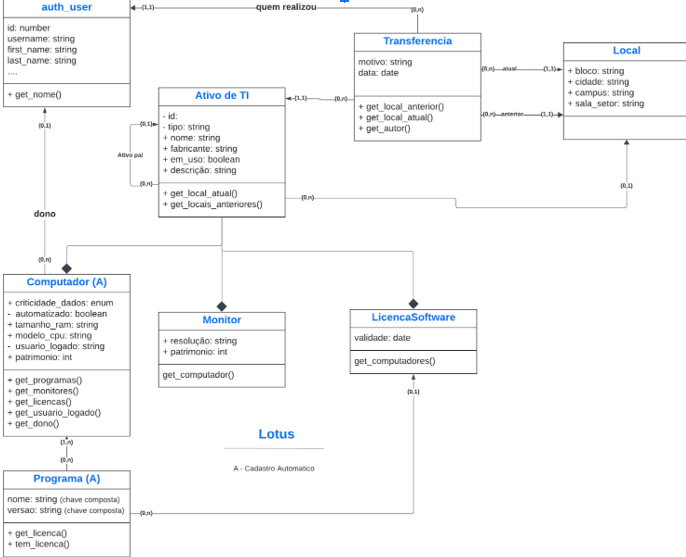
\includegraphics[width=0.8\linewidth]{figuras/diagramaclasses.png}
    \caption{Diagrama de classes}
    \label{fig:classes}
\end{figure}

Conforme ilustrado na Figura \ref{fig:classes} acima, optamos por uma abordagem simplificada de classes para mitigar a complexidade no sistema, especialmente devido ao tempo limitado previsto no cronograma de implementação.

\subsection{Diagrama Entidade-Relacionamento (ER)}
O Diagrama Entidade-Relacionamento (ER) é uma representação visual que mostra como os dados estão relacionados em um sistema. Ele modela entidades (objetos ou conceitos importantes para o sistema) e seus relacionamentos. Cada entidade tem atributos que representam suas propriedades, e as relações entre as entidades indicam como elas interagem entre si. O objetivo do diagrama ER é ajudar no planejamento e compreensão da estrutura do banco de dados, facilitando o design e a implementação.

\begin{figure}[H]
    \centering
    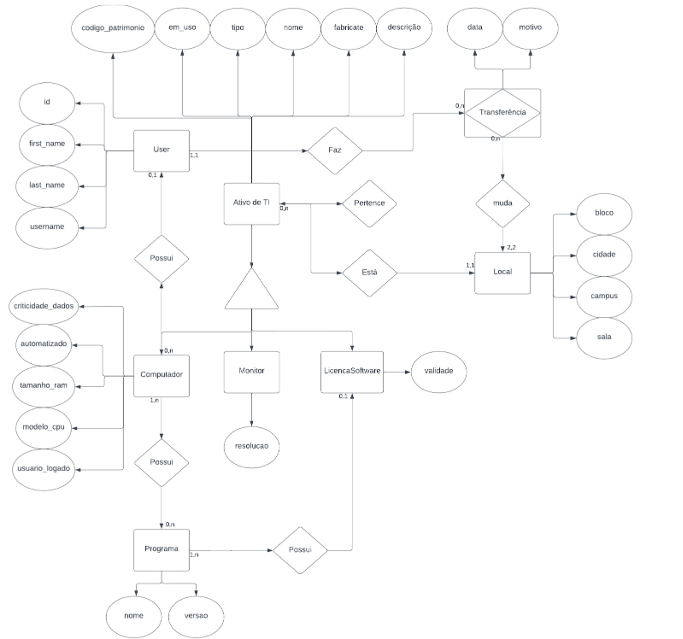
\includegraphics[width=0.8\linewidth]{figuras/DIAGRAMAer.png}
    \caption{Diagrama ER}
    \label{fig:classes}
\end{figure}


\section{Wireframe Front-End Desktop}
Este protótipo exibe todos os ativos cadastrados no sistema, organizados em uma lista com as principais informações de cada item.

\begin{figure}[H]
    \centering
    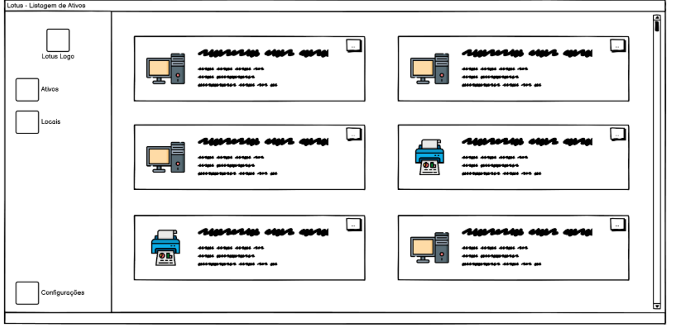
\includegraphics[width=1\linewidth]{figuras/lsitagemativos.png}
    \caption{Listagem de ativos}
    \label{fig:mockup1}
\end{figure}

Ao selecionar um ativo na listagem, esta interface apresenta informações detalhadas sobre o ativo, incluindo descrição, localização e relações com outros ativos.


\begin{figure}[H]
    \centering
    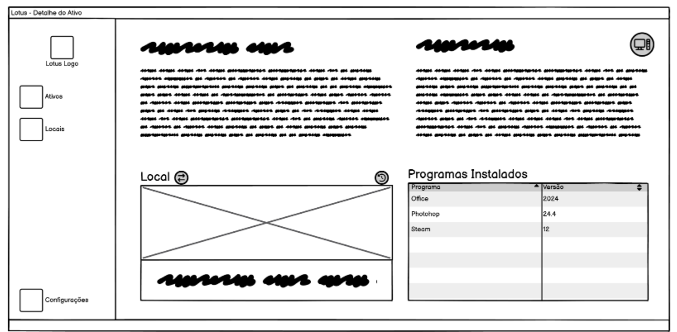
\includegraphics[width=1\linewidth]{figuras/detalhesativo.png}
    \caption{Detalhes do Ativo}
    \label{fig:mockup2}
\end{figure}

Neste modal, o usuário poderá alterar a localização de um ativo específico. A funcionalidade permite a rápida atualização da posição de um ativo no sistema.


\begin{figure}[H]
    \centering
    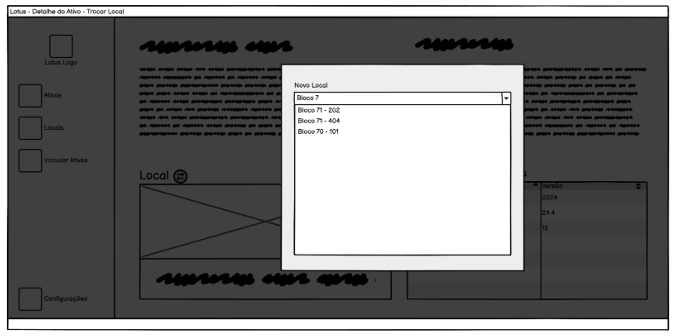
\includegraphics[width=1\linewidth]{figuras/trocarativo.png}
    \caption{Trocar Local do Ativo}
    \label{fig:mockup3}
\end{figure}

Este modal possibilita a associação entre diferentes ativos, formando grupos lógicos. A vinculação facilita o gerenciamento de ativos relacionados.


\begin{figure}[H]
    \centering
    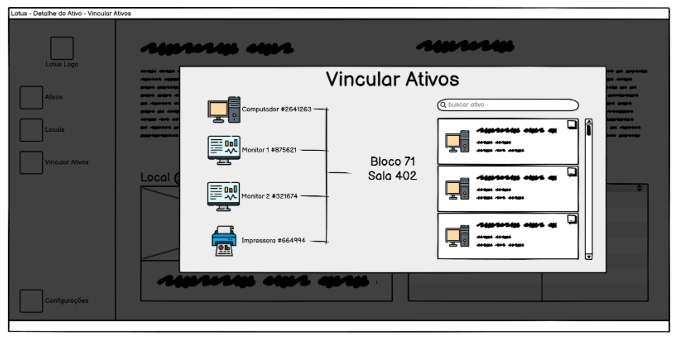
\includegraphics[width=1\linewidth]{figuras/vincularativo.png}
    \caption{Vincular Ativos}
    \label{fig:mockup3}
\end{figure}

Neste protótipo, o usuário pode visualizar todos os locais registrados no sistema, organizados de forma clara para facilitar a navegação e busca.


\begin{figure}[H]
    \centering
    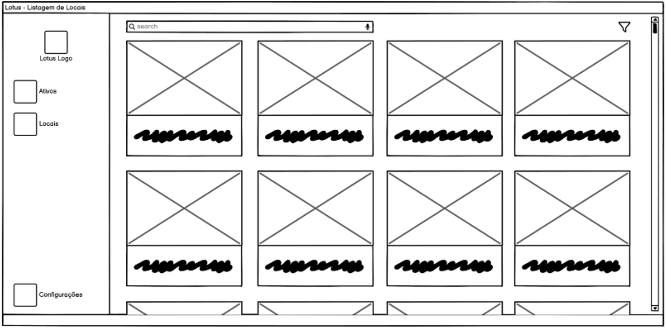
\includegraphics[width=1\linewidth]{figuras/listarlocais.png}
    \caption{Listagem de Locais}
    \label{fig:mockup3}
\end{figure}

Este protótipo oferece uma visão detalhada de um local específico. Inclui uma visualização espacial dos ativos alocados, exibindo sua posição em um mapa.

\begin{figure}[H]
    \centering
    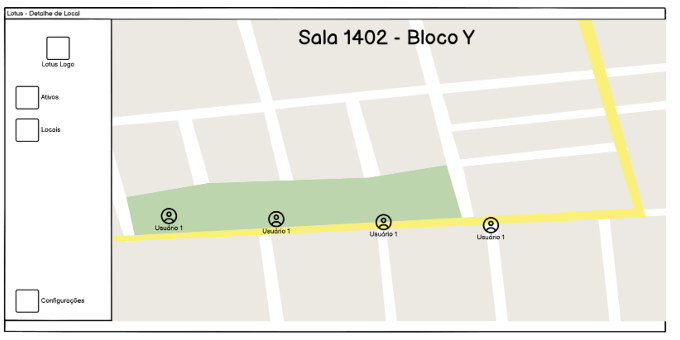
\includegraphics[width=1\linewidth]{figuras/detalheslocal.png}
    \caption{Detalhe de Local}
    \label{fig:mockup3}
\end{figure}


Optamos por criar alguns wireframes básicos para obtermos uma ideia inicial do design da nossa aplicação desktop. Esses wireframes são essenciais para visualizarmos como os diferentes elementos da interface serão organizados e interagirão entre si, antes de iniciarmos a implementação detalhada. Eles nos ajudarão a validar conceitos de usabilidade, identificar possíveis melhorias e alinhar expectativas sobre o visual e a funcionalidade da aplicação.




\section{Conclusão da Modelagem do Sistema}

Nesta etapa, detalhamos a modelagem do sistema, destacando as tecnologias básicas, a infraestrutura planejada e a estruturação do trabalho, incluindo o diagrama de classes.

\chapter{Implementação do Sistema}

Nessa etapa efetuamos a implementação do sistema e colocamos ele em produção. Isso envolveu definir as versões específicas das tecnologias e frameworks que serão utilizados para o desenvolvimento da aplicação. Essas escolhas são fundamentais para garantir compatibilidade, segurança e aproveitamento das últimas funcionalidades disponíveis.

\section{Front-End Web Desktop}
\begin{itemize}
\item Agurdando infos
\end{itemize}

\section{Agente Desktop}

\begin{itemize}
\item Golang 1.18.1
\end{itemize}



\section{Back-end Versões e Frameworks}
\begin{itemize}
\item Esperando Infos
\end{itemize}
\subsection{Banco de dados}
\begin{itemize}
\item Supabase (Banco de dados Postgres na nuvem)
\end{itemize}
\subsection{Hospedagem}
\begin{itemize}
\item A definir
\end{itemize}


\section{Implementação}

\begin{figure} [H]
    \centering
    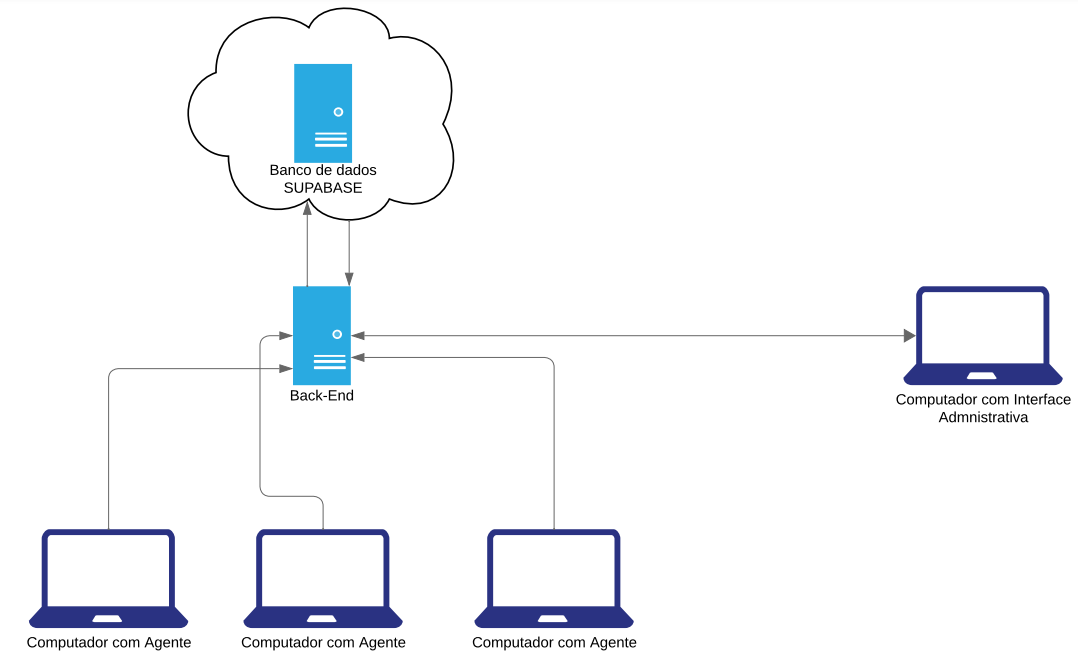
\includegraphics[width=1\linewidth]{figuras/INFRAIMPLE.png}
    \caption{Diagrama de implementação}
    \label{fig:diaimplementa}
\end{figure}
Na Figura \ref{fig:diaimplementa} Acima, pode-se observar como foi realizada a implementação com um back-end compartilhado para a interface de gerenciamento desktop e os agentes distribuídos. Para que o desenvolvimento de ambos os componentes ocorresse de maneira eficiente e integrada, foi necessário manter uma organização sólida entre o back-end e as funcionalidades específicas de cada parte do sistema.

\section{Geração de Dados Simulados}
Antes do início do desenvolvimento, as partes interessadas (Backend e Frontend e Agente) ajustaram previamente quais seriam os endpoints e as estruturas dos dados retornados pela API backend. Isso possibilitou a utilização de uma ferramenta chamada Mockaroo (https://www.mockaroo.com/), que serviu como um mock de dados e permitiu que as partes trabalhassem simultaneamente sem a dependência uma da outra.

Apenas no final do processo, as partes se juntaram para realizar uma parte da validação, garantindo que a conexão entre as partes não disparasse nenhum erro, independentemente do ambiente no qual o código estava sendo executado.

A outra parte da validação foi feita manualmente, com o acesso às telas buscando por caminhos diferentes para garantir que nenhum cenário fosse capaz de quebrar a aplicação.

\begin{figure}[H]
    \centering
    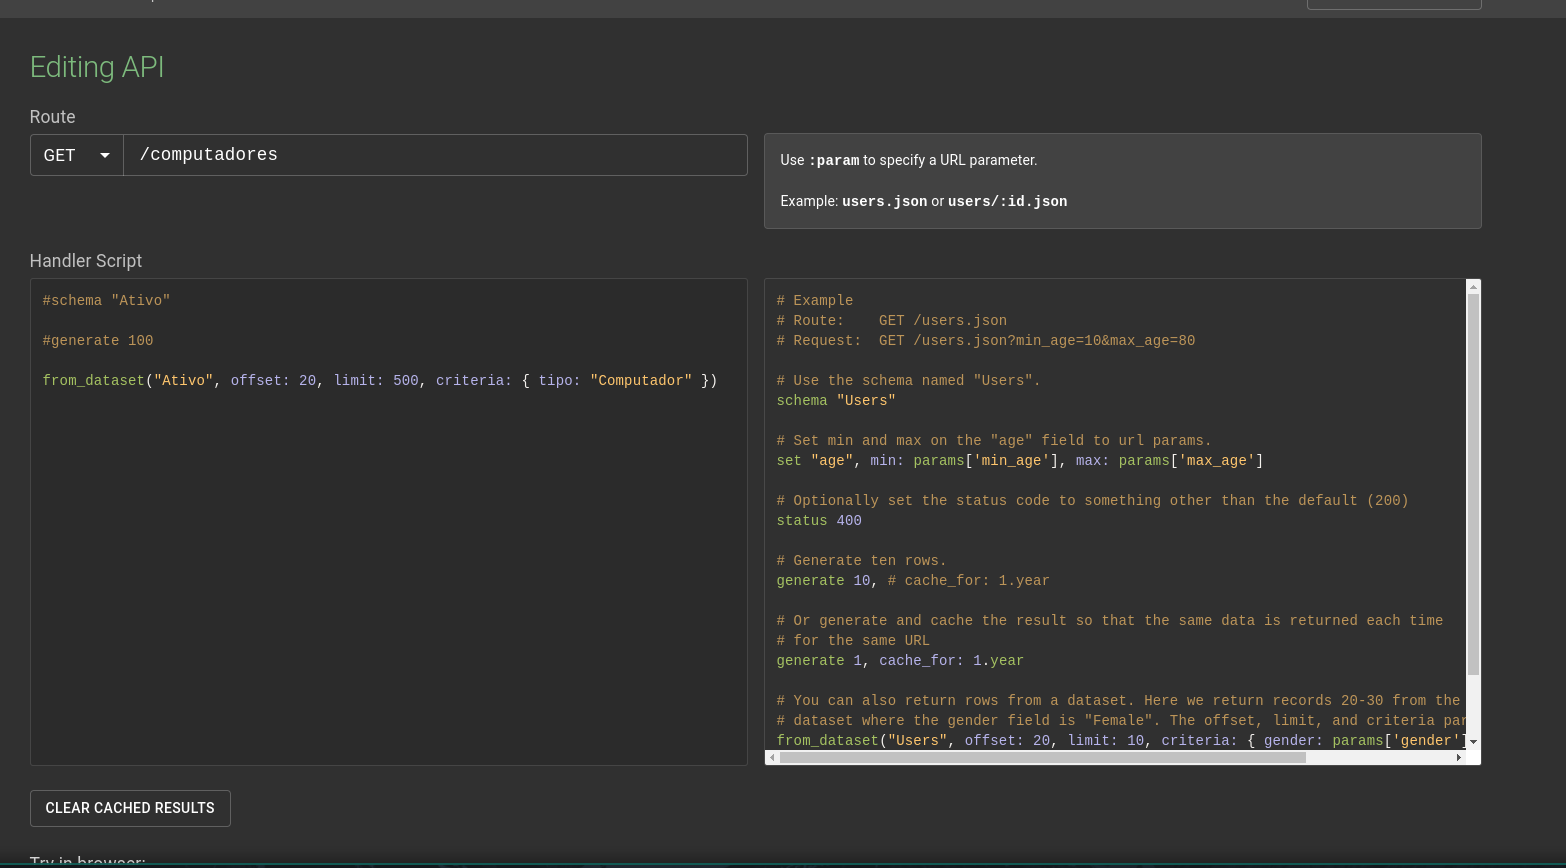
\includegraphics[width=0.6\linewidth]{figuras/apicomputador.png}
    \caption{Geração de requisições no mockaroo}
    \label{fig:enter-label}
\end{figure}

\begin{figure}[H]
    \centering
    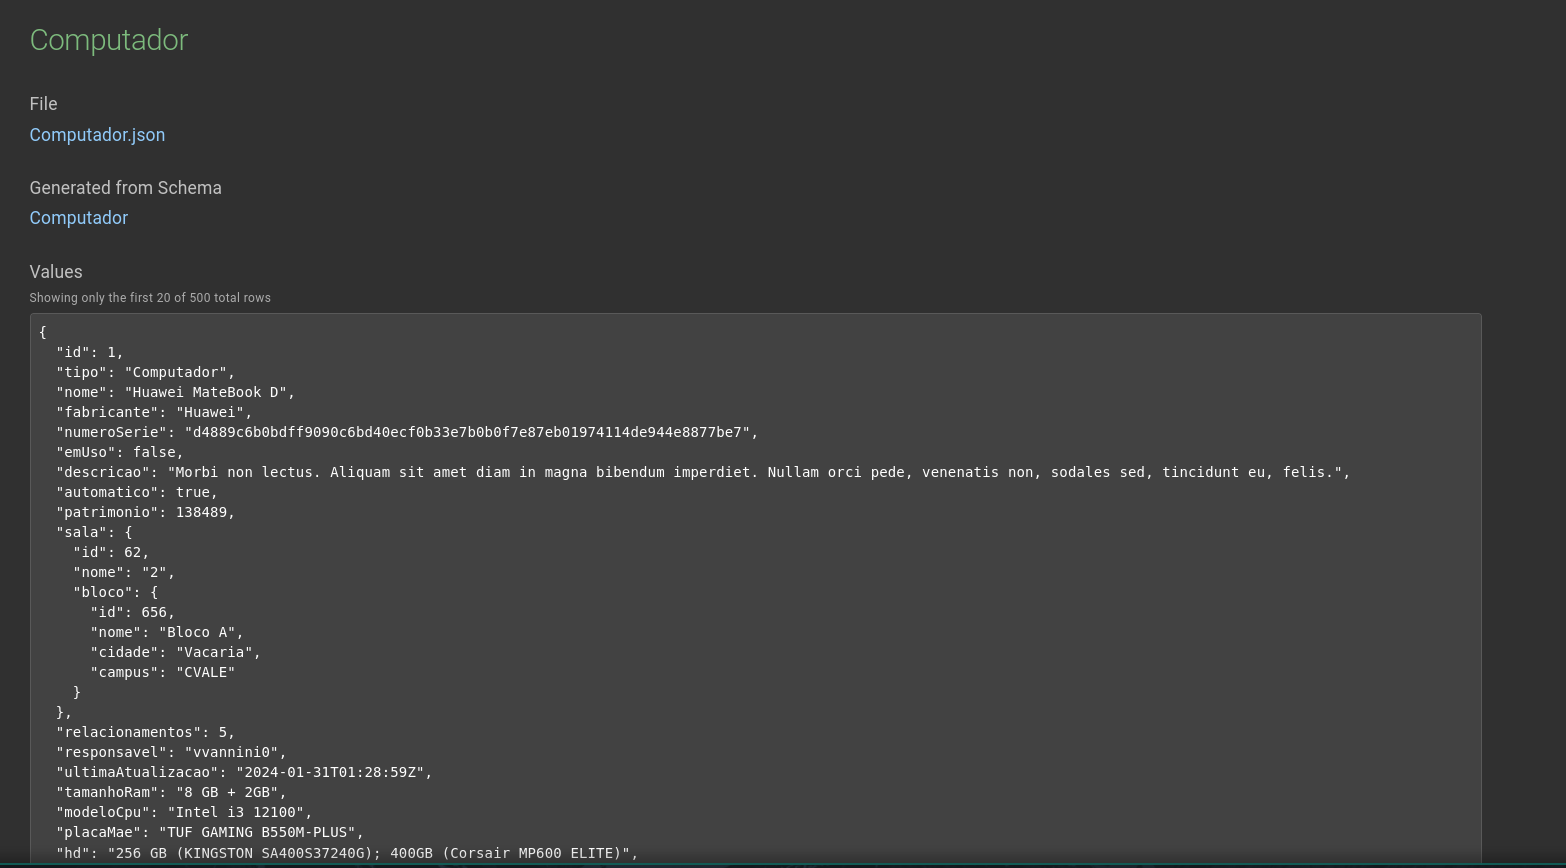
\includegraphics[width=0.6\linewidth]{figuras/mockcomputador.png}
    \caption{Exmplo de alguns formatos de dados}
    \label{fig:enter-label}
\end{figure}

Acreditamos que a utilização e organização com o Mockaroo foi essencial para que o desenvolvimento front-end e back-end e Agente pudesse ocorrer simultaneamente, sem que um dependesse do outro. O Mockaroo criou uma API com dados simulados, permitindo que o front-end realizasse testes e o back-end tivesse uma noção precisa de como deveria enviar os dados.

\section{Ferramentas para Utilização do Usuário}
\subsection{Interface Administrativa}
\begin{itemize}
\item Windows 10/11 e Linux
\end{itemize}
\subsection{Agente Desktop}
\begin{itemize}
\item Windows 10 /11 com o Powershell Atualizado
\end{itemize}


\section{Implementação Front-End Web}
Na criação da nossa aplicação web, nosso objetivo principal era exibir informações, com um foco significativo no design e na funcionalidade administrativa para adicionar e gerenciamento de conteúdo. Priorizamos especialmente a versão inicial para dispositivos móveis, garantindo exibições completas de todas as funcionalidades.



\subsection{Tela Principal}

\begin{figure}[H]
    \centering
    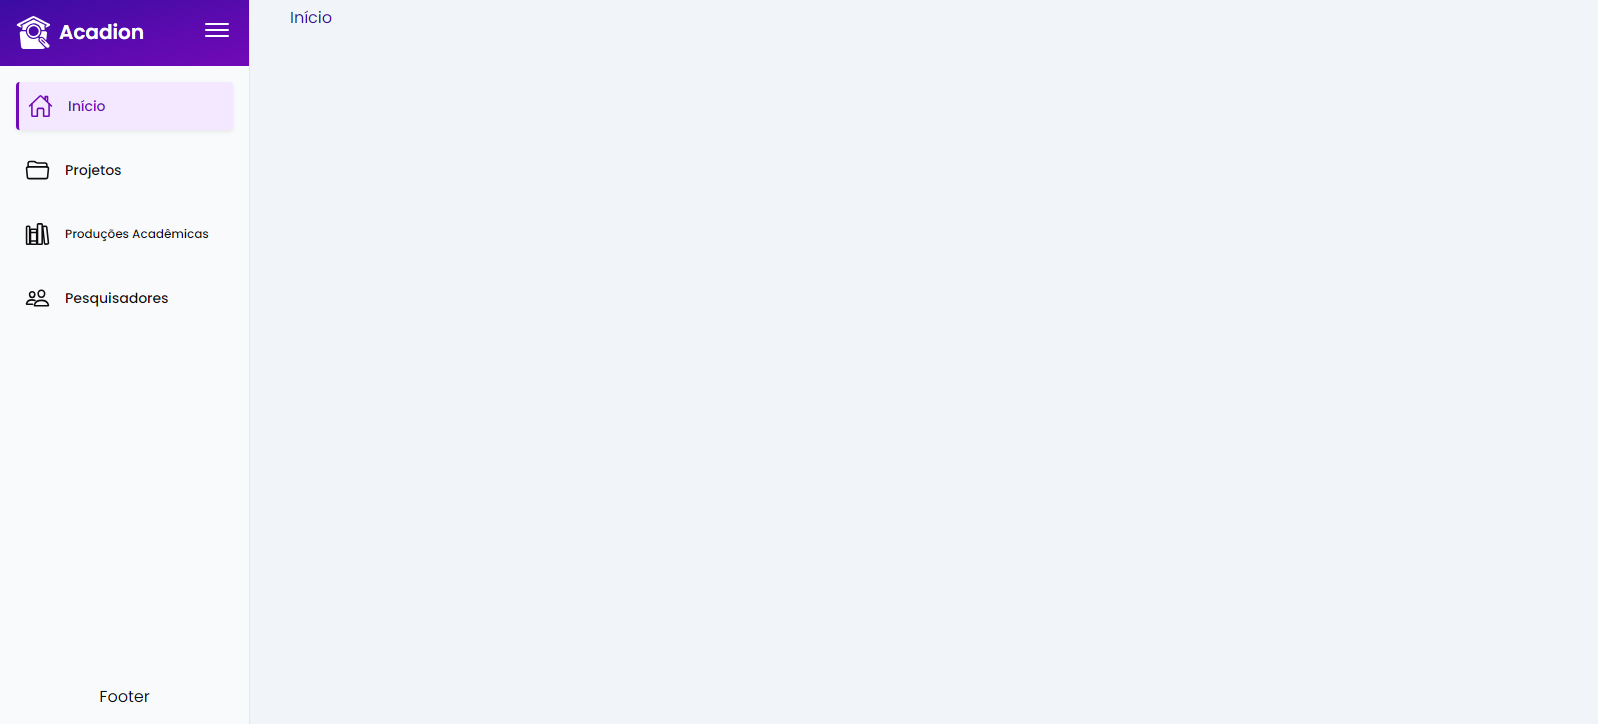
\includegraphics[width=1\linewidth]{figuras/SiteTelaPrincipal.png}
    \caption{Tela Início Web}
    \label{fig:enter-label}
\end{figure}
Optamos por focar nas funcionalidades principais, deixando propositalmente a implementação da tela inicial para um momento posterior.

\subsection{Tela Projetos}
\begin{figure}[H]
    \centering
    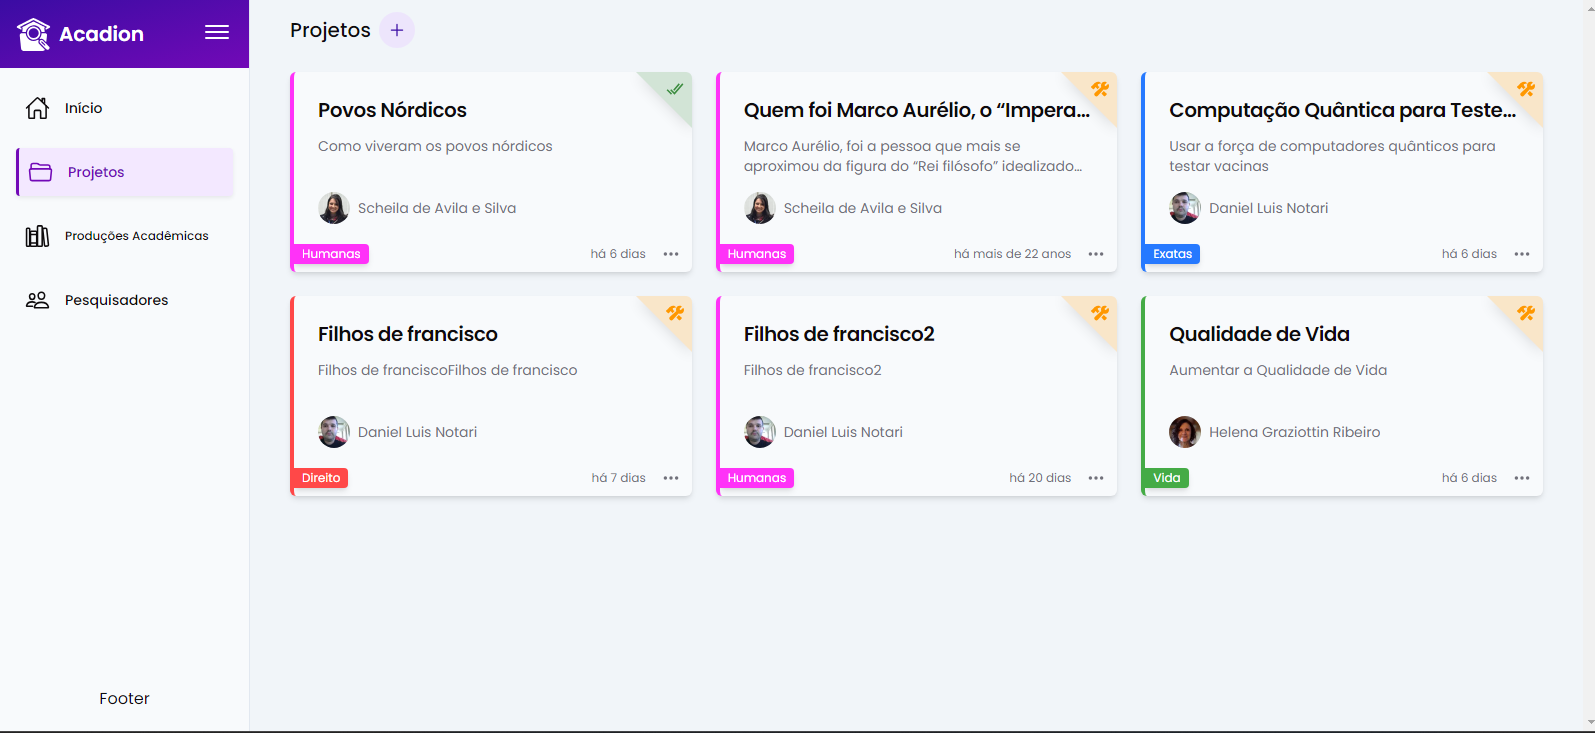
\includegraphics[width=1\linewidth]{figuras/TelaWebProjetos.png}
    \caption{Listagem dos projetos}
    \label{fig:projsweb}
\end{figure}
Nesta tela figura \ref{fig:projsweb}, são exibidos todos os projetos, mostrando o nome, um breve resumo e o coordenador de cada um. Além disso, é apresentada a área principal do projeto e seu status.

\begin{figure}[H]
    \centering
    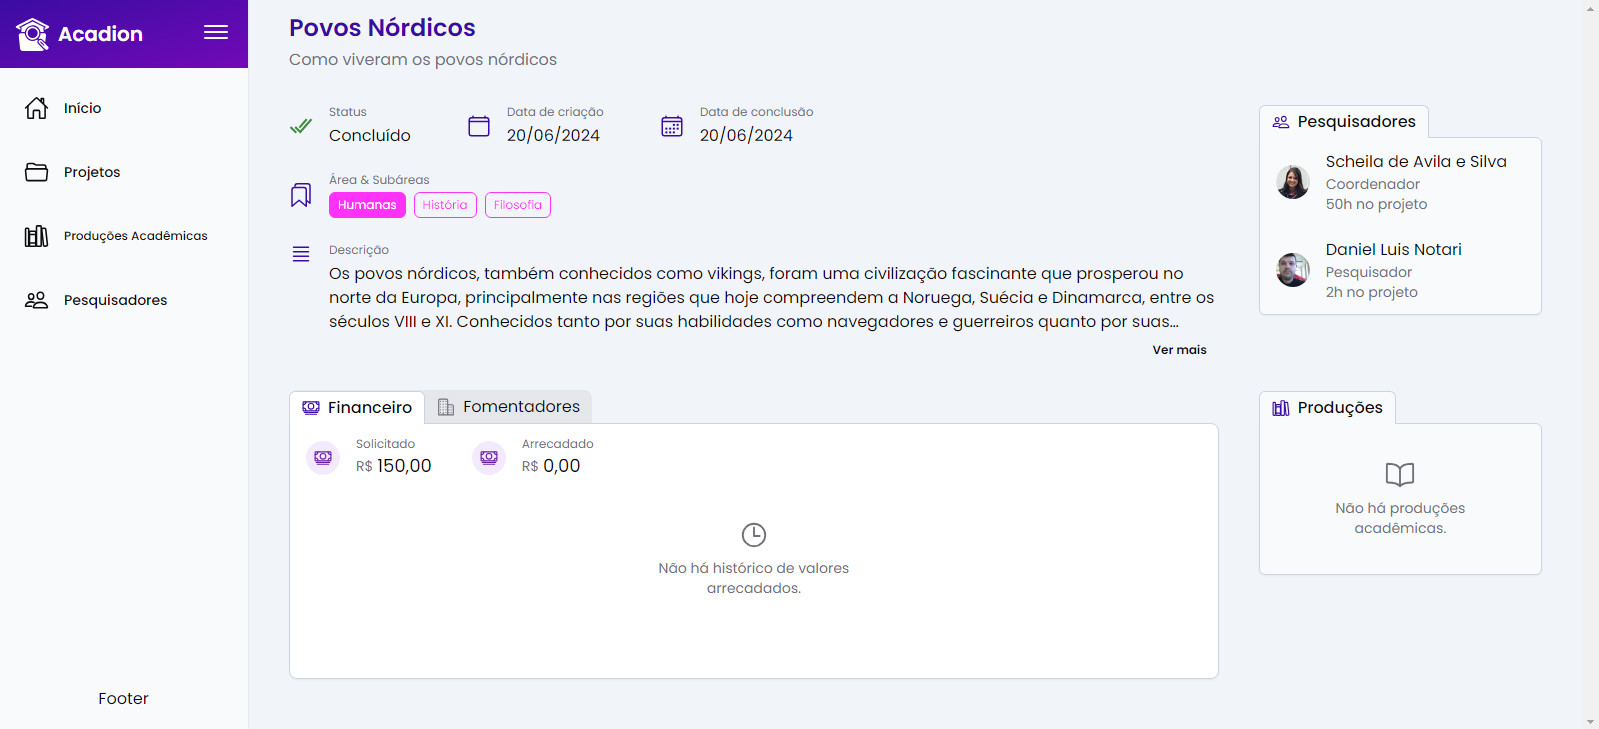
\includegraphics[width=1\linewidth]{figuras/DentroDeProjetos.png}
    \caption{Detalhes do projeto}
    \label{fig:detprojsweb}
\end{figure}
Nesta tela figura \ref{fig:detprojsweb}, são exibidos os detalhes do projeto selecionado, mostrando seu status, data de criação e conclusão. Também são apresentados todos os pesquisadores envolvidos, suas produções publicadas e a parte financeira, incluindo seus fomentadores.

\subsection{Adição de um Novo Projeto}
\begin{figure}[H]
    \centering
    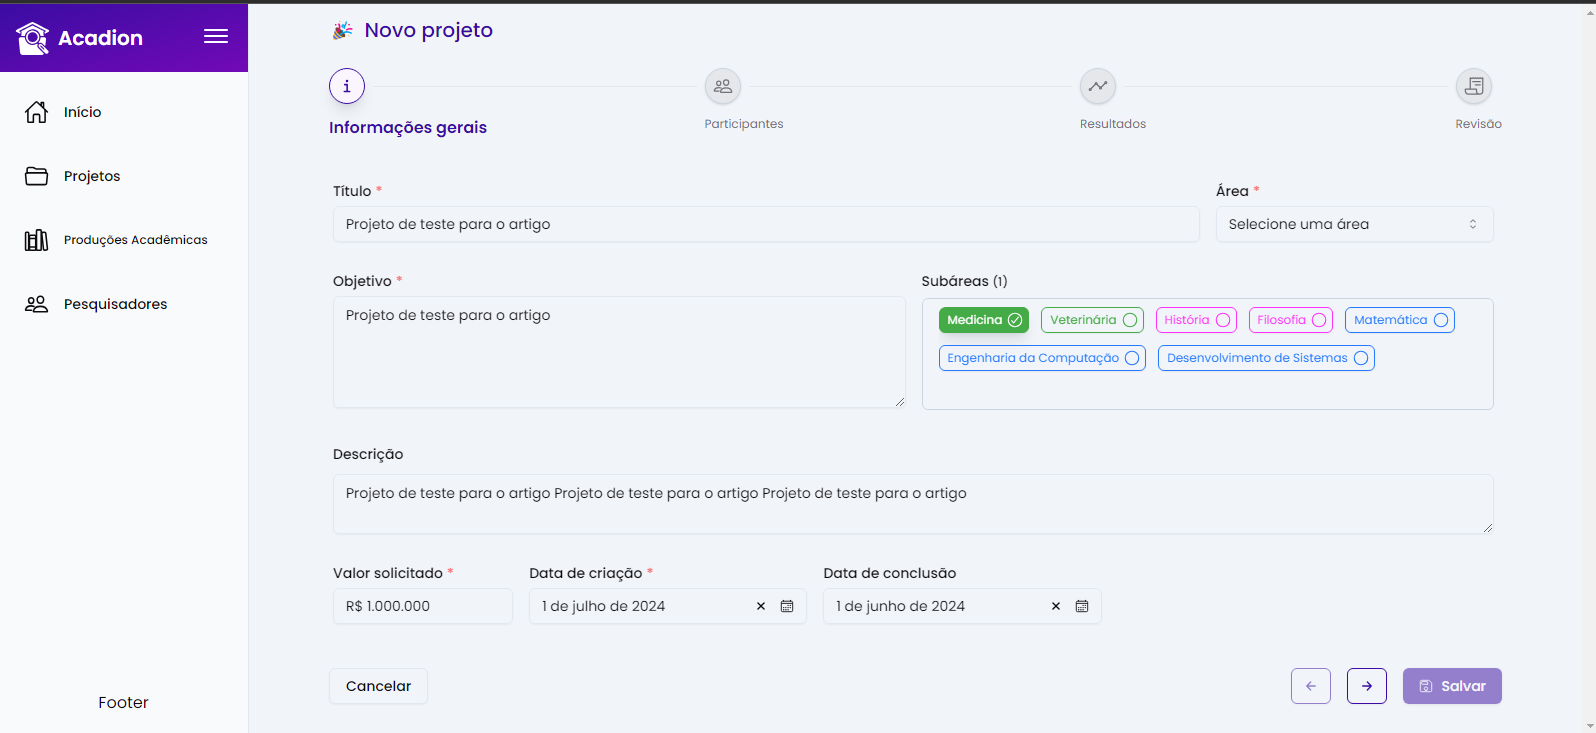
\includegraphics[width=1\linewidth]{figuras/NovoProjetoIG.png}
    \caption{Novo Projeto Informações gerais}
    \label{fig:addnewprojweb}
\end{figure}

\begin{figure}[H]
    \centering
    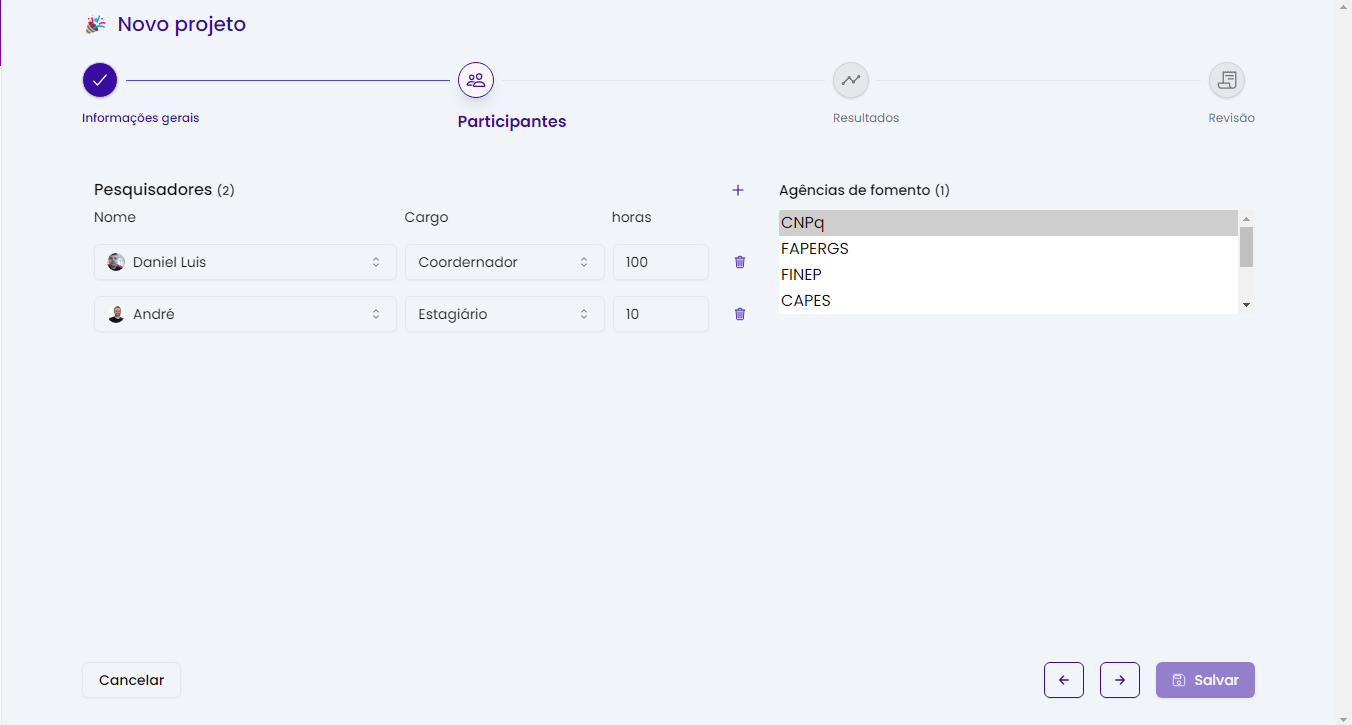
\includegraphics[width=1\linewidth]{figuras/NovoPorjetoParti.png}
    \caption{Novo Projeto Participantes}
    \label{fig:enter-label}
\end{figure}
\begin{figure}[H]
    \centering
    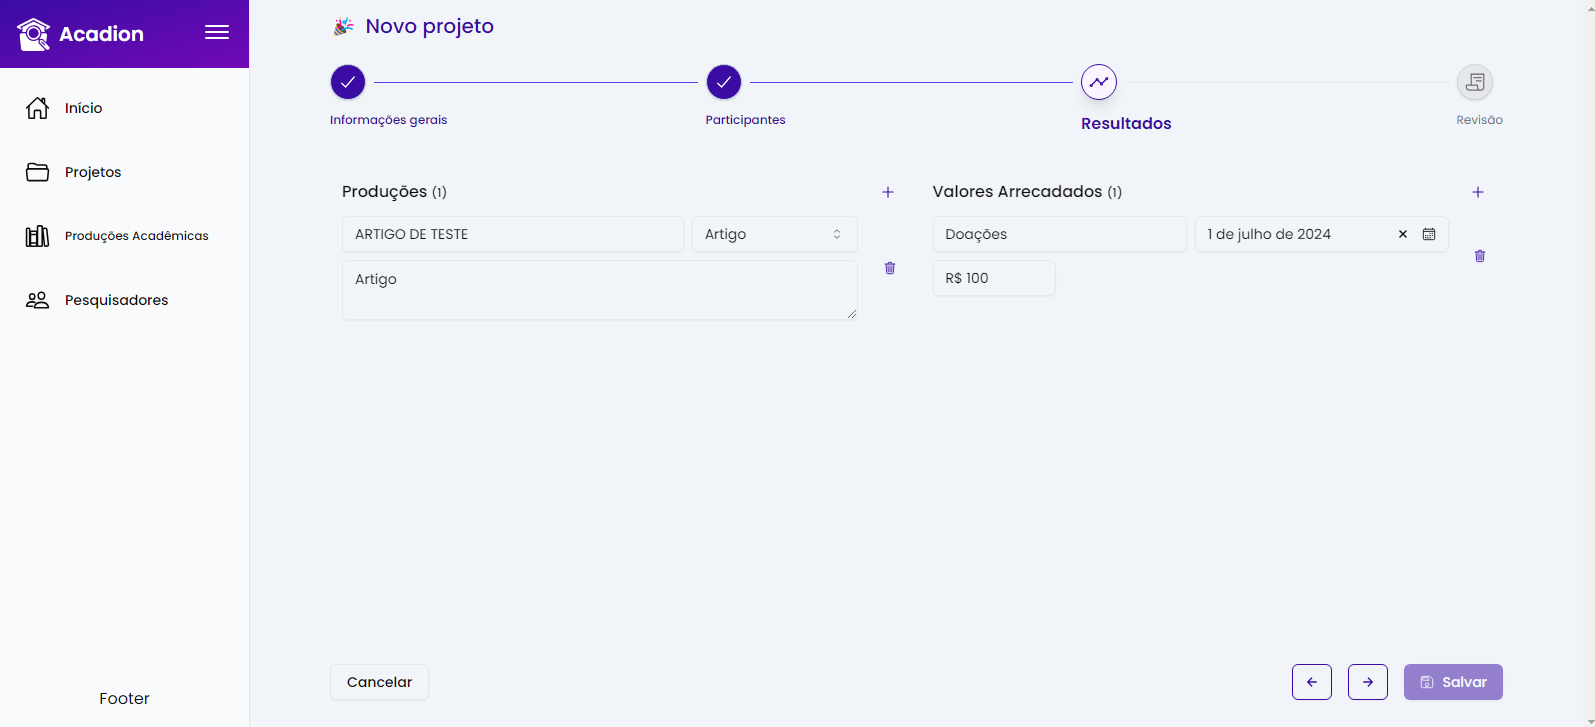
\includegraphics[width=1\linewidth]{figuras/NovoPorjetoResultados.png}
    \caption{Novo Projeto Resultados}
    \label{fig:enter-label}
\end{figure}

\begin{figure}[H]
    \centering
    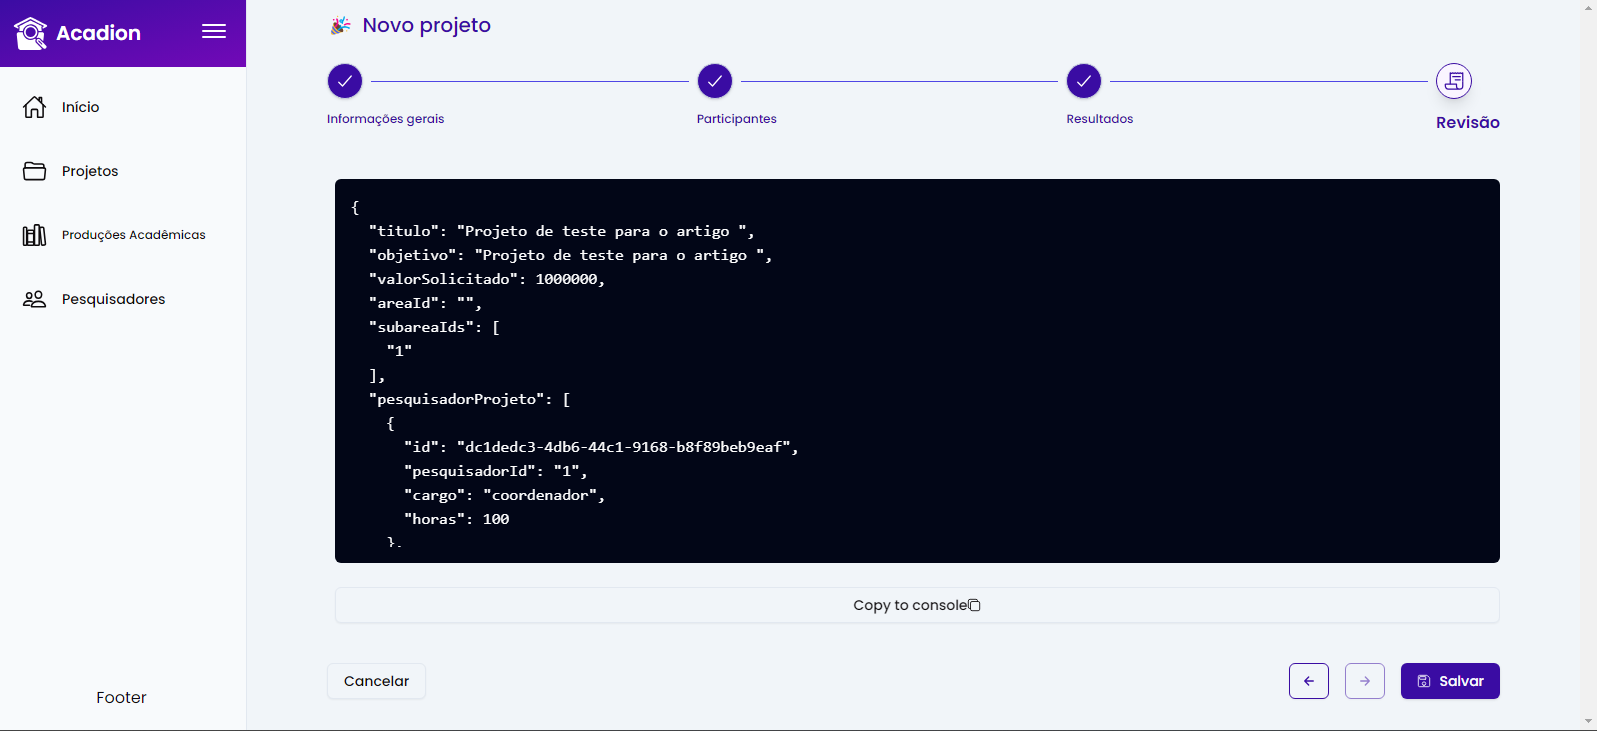
\includegraphics[width=1\linewidth]{figuras/NovoProjetoRevisao.png}
    \caption{Novo Projeto Revisão}
    \label{fig:enter-label}
\end{figure}

\begin{figure}[H]
    \centering
    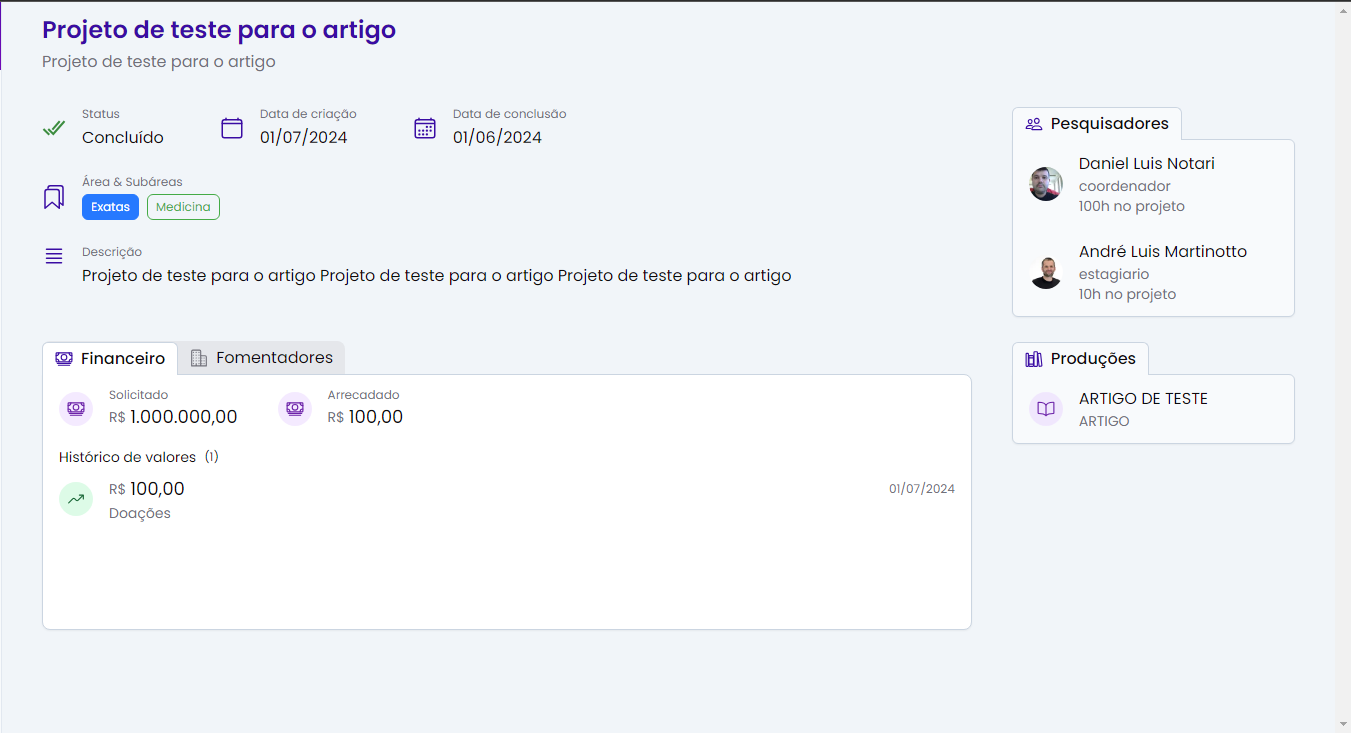
\includegraphics[width=1\linewidth]{figuras/NovoProjeto.png}
    \caption{Apos salvar o novo Projeto}
    \label{fig:newprojcreateweb}
\end{figure}

Após completar essas etapas das figuras \ref{fig:addnewprojweb} a \ref{fig:newprojcreateweb}, conseguimos salvar o projeto criado e adicioná-lo à lista de projetos.
\subsection{Acesso do Site}
URL: \hyperlink{https://acadion.vercel.app/}{https://acadion.vercel.app/}

\subsection{Observações da Implementação Web}
Algumas partes específicas da visualização de pesquisas ou de alguma produção acadêmica não foram implementadas nesta fase. No entanto, conseguimos criar e gerenciar projetos, incluindo suas publicações, dentro da aplicação web, dado o tempo disponível para a implementação.
Esta versão destaca o sucesso alcançado na implementação, enfatizando a fluidez e o design agradável obtidos. Para tornar o gerenciamento de dados viável, foi implementado um sistema rigoroso de validação no frontend.

\section{Implementação do Agente Desktop}

Durante o desenvolvimento do agente desktop, enfrentamos diversos desafios, tanto técnicos quanto conceituais. Um dos principais obstáculos foi aprender a linguagem Go (Golang), que foi escolhida pela sua eficiência e suporte nativo para concorrência. Além disso, foi necessário dominar o uso de \textit{Design Patterns} e implementar uma arquitetura \textit{N-tier} que atendesse aos requisitos de modularidade, escalabilidade e segurança do sistema.

Outro fator desafiador foi entender como implementar corretamente o agente para execução no sistema operacional Windows. Isso incluiu determinar a melhor forma de configurar o aplicativo para iniciar automaticamente com o sistema, sem interferir na experiência do usuário, e garantir que apenas uma instância do agente fosse executada por dispositivo.

A captação das informações foi outro ponto crítico. Era necessário que o agente coletasse dados como patrimônio, usuário logado e status do dispositivo, além de reportar essas informações de maneira eficiente e segura ao servidor. Implementar essa funcionalidade exigiu extensivas pesquisas e testes para garantir que o envio de dados fosse confiável e com baixo impacto no desempenho do sistema.

Além disso, trabalhamos na otimização do agente para operar de forma contínua sem causar sobrecarga no dispositivo ou na rede. Para isso, foram aplicados testes de desempenho e ajustes nos intervalos de coleta e envio de dados, garantindo um equilíbrio entre frequência de atualização e uso de recursos.

Embora desafiador, esse processo foi essencial para garantir que o agente desktop se integrasse perfeitamente ao restante do sistema, cumprindo seu papel de coletar e enviar informações em tempo real de maneira eficiente e segura.

\subsection{Arquitetura N-Tier do Agente}

A escolha pela Arquitetura \textit{N-Tier}, em vez de utilizar uma arquitetura em camadas convencional, como o \textit{Model-View-Controller} (MVC), foi motivada pelas especificidades do projeto de construção do agente. Diferentemente de sistemas web tradicionais, o agente desktop possui características e requisitos únicos, como a necessidade de comunicação direta e eficiente com o servidor, além da coleta e envio contínuos de dados.  

Dessa forma, optamos por projetar nossas próprias camadas, garantindo que cada parte do sistema estivesse alinhada às demandas do projeto e oferecendo maior flexibilidade para atender aos objetivos de desempenho, modularidade e escalabilidade.

\begin{figure}[H]
    \centering
    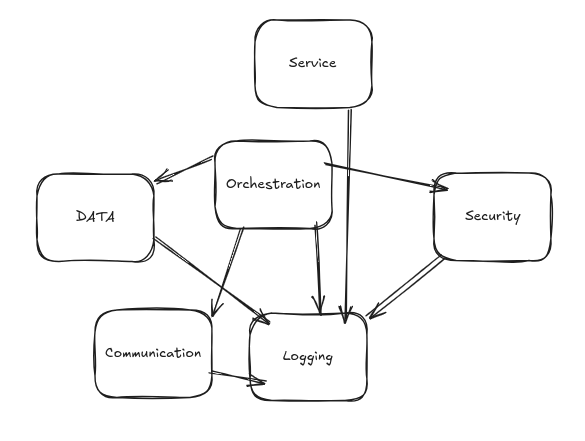
\includegraphics[width=1\linewidth]{figuras/NtierAgente.png}
    \caption{N-Tier Agente}
    \label{fig:NTagente}
\end{figure}

Na Figura: \ref{fig:NTagente} observamos o desenho das camadas que compõem a arquitetura do agente desktop. Cada camada possui responsabilidades bem definidas, conforme descrito abaixo:

\begin{itemize}
    \item \textbf{Service:} Responsável por criar e garantir que o agente seja executado como um serviço. Para isso, utilizamos a biblioteca \textit{Kardianos Service} em Golang, que facilita a configuração e o gerenciamento do serviço no sistema operacional.
    
    \item \textbf{Security:} Camada dedicada às funções de segurança. Atualmente, é responsável pela aplicação de HMAC nos \textit{JSONs}, garantindo a integridade e a autenticidade dos dados enviados ao servidor.
    
    \item \textbf{Logging:} Implementa um sistema de \textit{log} centralizado para capturar erros e informações relevantes da aplicação, permitindo o monitoramento eficiente e a depuração do sistema.
    
    \item \textbf{Data:} Camada encarregada da extração de informações do computador, como dados de hardware, IP, usuário logado e outras métricas relevantes.
    
    \item \textbf{Communication:} Cuida da comunicação com o \textit{back-end}, estabelecendo conexões seguras e confiáveis para enviar os dados coletados e receber respostas do servidor.
    
    \item \textbf{Orchestration:} A camada mais importante do agente, sendo responsável por integrar as demais camadas. Ela forma os \textit{JSONs}, aplica HMAC, coordena o envio para o servidor e organiza as funcionalidades para garantir o funcionamento harmonioso do sistema.
\end{itemize}
Em termos de autorização de comunicação entre as camadas, as seguintes regras foram definidas para garantir uma arquitetura modular e segura:

\begin{itemize}
    \item Todas as camadas têm permissão para acessar a camada \textbf{Logging}, permitindo o registro centralizado de erros e informações relevantes.
    \item A camada \textbf{Service} é isolada e não pode ser acessada por nenhuma outra camada, garantindo que sua funcionalidade seja protegida e executada apenas de forma controlada.
    \item A camada \textbf{Orchestration} possui permissões amplas, podendo acessar as camadas \textbf{Data}, \textbf{Communication}, \textbf{Security} e \textbf{Logging}. Isso reflete seu papel central na integração e coordenação das funcionalidades do agente.
\end{itemize}

Essa organização hierárquica das permissões reforça a modularidade do sistema, além de garantir que cada camada execute suas responsabilidades sem comprometer a segurança ou a integridade da aplicação.

\subsection{Design Patterns Utilizados no Agente}

De acordo com as diretrizes apresentadas por \textit{Refactoring Guru} (\url{https://refactoring.guru/design-patterns}), diversos \textit{Design Patterns} foram selecionados para a implementação do agente desktop, cada um atendendo a necessidades específicas do projeto. Os principais padrões aplicados foram:

\begin{itemize}
    \item \textbf{Singleton:} Utilizado para o objeto de \textit{Logging}, garantindo que apenas uma instância do sistema de registro de logs seja criada e utilizada por todo o programa, centralizando o controle e facilitando o monitoramento.

    \item \textbf{Factory:} Aplicado na criação de objetos responsáveis pela captura de informações do sistema, como dados de hardware e software. A \textit{Factory} verifica o sistema operacional (Windows ou Linux) e instancia os objetos apropriados para cada plataforma, garantindo flexibilidade e compatibilidade.

    \item \textbf{Builder:} Utilizado para a criação de \textit{JSONs}, permitindo construir de forma estruturada e modular as informações principais, como dados de \textit{Core}, programas instalados e especificações de hardware. Esse padrão facilita a adição de novos campos e melhora a manutenção do código.

    \item \textbf{Mediator:} Implementado na camada de \textit{Orchestration}, servindo como um intermediário para coordenar a comunicação e interação entre as diferentes camadas, como \textit{Data}, \textit{Security}, \textit{Communication} e \textit{Logging}.
\end{itemize}

A aplicação desses \textit{Design Patterns} foi essencial para garantir a modularidade, escalabilidade e organização do código, além de permitir um desenvolvimento mais eficiente e alinhado às melhores práticas de engenharia de software.

\subsection{Implementação do Agente}

Inicialmente, o agente foi planejado para funcionar em sistemas operacionais Linux e Windows. No entanto, devido ao curto prazo de implementação, optamos por focar no seu funcionamento exclusivamente em Windows. Apesar disso, grande parte do programa foi estruturada para permitir futuras adaptações para Linux, utilizando abordagens como o \textit{Factory Pattern}, que facilita a criação de objetos específicos para diferentes sistemas operacionais.

O agente é distribuído como um executável (\texttt{.exe}) que é executado em sistemas Windows 10 e 11. O processo de instalação ocorre da seguinte forma:

\begin{enumerate}
    \item No diretório \texttt{C:/}, crie uma pasta com um nome de sua preferência.
    \item Copie o arquivo \texttt{agente.exe} para dentro dessa pasta.
    \item Abra o \textit{Prompt de Comando} como administrador.
    \item Navegue até a pasta criada e execute o comando \texttt{./agente.exe install}.
\end{enumerate}

Após essa etapa, o agente cria um serviço no Windows chamado \textbf{LOTUS}, configurado para iniciar automaticamente. Esse serviço permite que o agente opere de forma contínua e integrada com o restante do sistema, garantindo a coleta e envio de dados de forma eficiente e transparente.

\subsection{Segurança do Agente}

Atualmente, a segurança do agente está parcialmente implementada, com destaque para o uso do HMAC (Hash-based Message Authentication Code). Essa funcionalidade foi integrada ao agente para garantir a integridade e autenticidade dos \textit{JSONs} enviados ao servidor. No entanto, o suporte correspondente no \textit{back-end} ainda não foi concluído, limitando sua aplicação prática no momento.

Outras medidas de segurança, como a implementação de um sistema de autenticação baseado em tokens e a troca de chaves para criptografia, foram planejadas, mas não foram priorizadas devido ao curto prazo de desenvolvimento. Embora ainda não implementadas, essas funcionalidades estão previstas para futuras atualizações do sistema, visando melhorar significativamente a proteção dos dados e das comunicações.

Apesar dessas limitações iniciais, a arquitetura do agente foi projetada para facilitar a inclusão dessas melhorias de segurança no futuro, garantindo que o sistema possa evoluir para atender a requisitos mais robustos.


\subsection{Informações Extras do Agente}

Futuramente, está planejada a criação de uma camada de configuração para o agente, utilizando arquivos no formato YAML. Essa camada permitirá configurar informações como rotas e outros parâmetros essenciais, visando simplificar a manutenção e personalização do agente conforme as necessidades específicas de cada ambiente.

Além disso, dentro da pasta onde o agente é configurado como serviço, serão gerados os seguintes arquivos:

\begin{itemize}
    \item \textbf{Arquivos de Log:} Criados automaticamente para registrar erros, eventos e informações relevantes do funcionamento do agente, facilitando a análise e depuração do sistema.
    \item \textbf{Arquivo \texttt{pat.txt}:} Esse arquivo armazena o patrimônio do computador, que é capturado a partir do nome da máquina. Caso o nome não contenha o número de patrimônio, será gerado automaticamente um número negativo aleatório como identificador.
\end{itemize}

Essas funcionalidades adicionais visam tornar o agente mais autossuficiente e adaptável, além de facilitar seu gerenciamento em ambientes distribuídos.
 



\section{Implementação do Back-end}
A aplicação adota o padrão MVC (Model-View-Controller), onde cada camada desempenha um papel fundamental na organização e funcionalidade do sistema. Na camada Model, localizada nos arquivos models.py, reside a estrutura de dados e a lógica de negócios, mapeando diretamente para tabelas do banco de dados. A camada View, implementada em views.py, cuida da apresentação e da lógica de controle, respondendo às chamadas de endpoints e processando dados para retorno apropriado. O Controller é gerenciado pelo Django por meio do URL dispatcher em urls.py, roteando requisições para as views corretas. Adicionalmente, Serializers são utilizados para converter modelos em instâncias JSON, facilitando a comunicação entre o backend e os clientes da API. Essa divisão estruturada não apenas organiza o código de maneira lógica, mas também promove escalabilidade e manutenção simplificada, permitindo o desenvolvimento e teste independentes de cada camada.

\subsection{Deploy do Back-end em nuvem}

Para o deployment da aplicação, optamos pelo serviço Cloud Run da Google Cloud Platform. Esse serviço oferece a flexibilidade necessária para executar containers de maneira escalável e automatizada. Inicialmente, configuramos um Dockerfile para definir o ambiente de execução da aplicação. Além disso, desenvolvemos scripts bash auxiliares que garantem a inicialização automática do servidor da aplicação ao iniciar o container, configurando a exposição da porta correta e outras configurações necessárias.

Adotamos também um webhook de integração contínua com o repositório GitHub. Esse webhook é configurado para acionar automaticamente o build de um novo container sempre que há um merge na branch principal do projeto. Essa prática assegura que o ambiente de produção esteja constantemente atualizado com as últimas alterações do código-fonte, minimizando a necessidade de intervenção manual e aumentando a eficiência do processo de deployment.

Para garantir a segurança e configurar variáveis de ambiente, utilizamos a interface intuitiva fornecida pelo console da Google Cloud Platform. Isso nos permitiu definir variáveis sensíveis de forma segura e aplicar configurações de segurança de tráfego diretamente na plataforma.
\section{Github para o Codigo Fonte}
https://github.com/Projetos-Faculdade-UCS/Projac

\section{Conclução da Implementação}
Em resumo, a implementação do backend foi um sucesso, com a aplicação sendo eficientemente hospedada na nuvem através do Google Cloud em containers Docker, oferecendo uma API robusta para ser consumida por aplicativos e servidores web. O aplicativo móvel foi completamente implementado, integrando todas as funcionalidades planejadas e proporcionando uma experiência de usuário completa. Embora o desenvolvimento da versão web não tenha sido concluído integralmente, conseguimos alcançar nossos objetivos principais, incluindo o cadastro de pesquisas e a apresentação de um design moderno e funcional.

\section{



































\chapter{CONSIDERAÇÕES FINAIS}


Este trabalho abordou o desenvolvimento de um software para centralização e gestão de dados acadêmicos, com o objetivo de melhorar a organização, acessibilidade e utilização do conhecimento gerado por pesquisas e projetos em instituições de ensino e pesquisa. Através da integração de metodologias ágeis como TDD e BDD, foi possível criar uma solução tecnológica robusta e adaptável, capaz de atender às necessidades específicas de diferentes usuários, desde estudantes até gestores acadêmicos.

A implementação de tecnologias modernas para o desenvolvimento do Front-end (React e Flutter) e Back-end (Python e Django), bem como o uso de bancos de dados em nuvem, proporcionou uma base sólida para a criação de um sistema escalável e seguro. A arquitetura do sistema, detalhada ao longo do trabalho, demonstrou como diferentes componentes podem interagir de maneira eficiente para garantir a integridade e a confiabilidade dos dados.

Os testes realizados ao longo do desenvolvimento garantiram a qualidade do software, validando suas funcionalidades e assegurando que o sistema atendesse aos requisitos especificados. A abordagem modular adotada permitiu uma maior flexibilidade na implementação e na manutenção do sistema, facilitando futuras expansões e melhorias.

Como principais contribuições, destacam-se:
\begin{itemize}
    \item A centralização de dados acadêmicos em um único repositório acessível, evitando a duplicação de esforços e promovendo a colaboração entre pesquisadores.
    \item A facilitação da combinação e análise de dados, potencializando a descoberta de novas soluções e insights.
    \item A promoção de um ambiente colaborativo e inovador, incentivando a integração entre diferentes plataformas e dispositivos.
\end{itemize}

Em conclusão, o desenvolvimento deste software representa um avanço significativo na gestão de dados acadêmicos, proporcionando uma plataforma eficiente e intuitiva que beneficia toda a comunidade acadêmica.



    

    
\include{2-textuais/4-Referencias}
%\include{2-textuais/nomedoarquivo sem .tex}
%\include{2-textuais/nomedoarquivo sem .tex}

%=======================================================================
% ELEMENTOS PÓS-TEXTUAIS
%=======================================================================
\postextual

% ----------------------------------------------------------------------
% Referências bibliográficas
% ----------------------------------------------------------------------
\bibliographystyle{abntex2-alf}
\bibliography{3-pos-textuais/referencias}


% ----------------------------------------------------------------------
% Apêndices (se necessário)
% ----------------------------------------------------------------------
%\begin{apendicesenv}
	
	% ----------------------------------------------------------
	%\chapter{Título do Apêndice}
	%\label{apendice:exemplo} 
    % ----------------------------------------------------------

	% ----------------------------------------------------------
	%chapter{Outro Apêndice }
	%\label{apendice:exemplo2} 
	% ----------------------------------------------------------
	
\end{apendicesenv}

% ----------------------------------------------------------------------
% Anexos (se necessário)
% ----------------------------------------------------------------------
%% ---
% Inicia os anexos
% ---
\begin{anexosenv}

	% ----------------------------------------------------------
	%\chapter{Anexo ...}
	%\label{anexo:nomea} 
	% ----------------------------------------------------------
	

	% ----------------------------------------------------------
	%\chapter{Anexo ...}
	%\label{anexo:nomeb} 
	% ----------------------------------------------------------

\end{anexosenv}


\end{document}